\newpage
\section{Evaluierung des Prototyps}
Im Folgenden wird gezeigt welche funktionalen Anforderungen erfüllt werden. Auch wird ausgewertet, inwieweit die nicht funktionalen Anforderungen an die Benutzerfreundlichkeit und Effizienz erfüllt werden.

\subsection{Funktionale Anforderungen}\label{sec:EvaluationFunctionalRequirements}
Im Abschnitt \ref{sec:FunctionalRequirements} werden die funktionalen Anforderungen erläutert. Die meisten dieser Anforderungen werden durch den Prototyp erfüllt, weshalb hier nur die nicht erfüllten Anforderungen erwähnt werden. Bei dem Prototyp handelt es sich zwar – wie in den Anforderungen definiert – um eine responsive Webanwendung, sie funktioniert allerdings nicht auf allen Geräten vollständig. So können die für die Gebäudemodelle genutzten \ac{glTF}-Modelle nicht im Safari-Browser angezeigt werden, weil die Modelle das \ac{WebP} Bildformat für die Texturen nutzen und dieses noch nicht vollständig von Safari unterstützt wird \cite{CanIUseWebP}. Da es sich hierbei um eine Beschränkung des Safari-Browsers handelt, die in Zukunft von Apple behoben werden sollte und weil alle anderen Funktionen des Prototyps auch im Safari-Browser funktionieren, wurde hierfür kein Workaround entwickelt. Während die Positionsänderungen der Roboter animiert werden, ist das bei den Rotationsänderungen aufgrund eines Bugs nicht der Fall. Aus diesem Grund ist die Anforderung, dass der Roboter in der Übersicht fährt, nicht vollständig, aber ausreichend erfüllt.

Die Anforderungen an die Methode zur Gebäudemodell-Generierung konnten mit dem Einsatz des \ac{LiDAR}-Scannens weitestgehend erfüllt werden. Zum Scannen wird ein neueres iPhone benötigt, welches ein Nutzer unter Umständen bereits besitzt. Das Generieren der Modelle erfordert wenig Aufwand, wobei dieser davon abhängig ist, wie gründlich gescannt wird. Insgesamt ist für das Scannen nur wenig Know-how nötig. Die entstandenen Modelle müssen für den Prototyp manuell komprimiert werden, wofür beispielsweise das im Abschnitt \ref{sec:ModelFileFormat} erwähnte Webtool OptimizeGLB infrage kommt. In einem Produktivsystem könnten die Modelle aber auch mithilfe des \ac{glTF}-Transform \ac{npm}-Pakets \cite{glTF-Transform} automatisch beim Import in den Editiermodus komprimiert werden. Zum einen variiert die Qualität der erzeugten Modelle dadurch wie gründlich die Scans durchgeführt wurden. Zum anderen variiert sie auch durch die eingesetzte Komprimierungsmethode. Insbesondere kleinere Ungenauigkeiten können in den erzeugten Modellen ignoriert werden, solange diese Ungenauigkeiten keinen Einfluss auf die Übersichtlichkeit des Modells haben.

\subsection{Benutzerfreundlichkeit}
Die Benutzerfreundlichkeit wird durch die Einhaltung der Usability Entscheidungsregeln gefördert und durch die Auswertung der Usability Tests bewertet. Beides wird im Folgenden genauer erörtert.

\subsubsection{Usability Entscheidungsregeln}\label{sec:UsabilityHeuristics}
Die Usability Entscheidungsregeln konnten weitestgehend eingehalten werden. Im Folgenden wird aufgezeigt wie ein paar Entscheidungsregeln konkret eingehalten werden.

Die erste Regel besagt, dass der Nutzer immer innerhalb einer angemessenen Zeitspanne durch geeignete Rückmeldungen mitbekommen sollte, was gerade passiert \cite[Regel 1]{Nielsen.1994}. Diese Regel wird durch verschiedene Features in der Übersicht und Steuerung erfüllt. Zum einen gibt es die Echtzeit-Aktualisierungen des Roboterstandorts und -Status über die \gls{Websocket}-Verbindung mit dem \ac{BCB}. Zum anderen werden Statusänderungen auch über die Farben der Buttons signalisiert. Außerdem gibt es einen Wait-Cursor, um Ladevorgänge anzuzeigen.

% Die zweite Regel erwartet, dass der Nutzer die Sprache der Anwendung versteht und somit beispielsweise möglichst wenig Fachsprache verwendet wird. In der Steuerung und Verwaltung gibt es nur wenig Text, da vor allem Icons eigesetzt werden. In der Verwaltungsansicht werden möglicherweise unklare Begriffe wie Ladestation über Tooltips erklärt. Außerdem werden Einstellungsänderungen über Dialoge erklärt.

Da Benutzer oft versehentlich Aktionen ausführen, gibt es die dritte Regel, die klar gekennzeichnete Abbruchoptionen fordert, damit unerwünschte Aktionen abgebrochen oder rückgängig gemacht werden können \cite[Regel 3]{Nielsen.1994}. Um die Kamera wieder in die Ausgangsposition zu bringen, wenn diese versehentlich an eine ungewünschte Position bewegt wurde, gibt es in der Übersicht einen entsprechenden Button. In der Steuerung gibt es außerdem einen Button, mit dem der aktuelle Lieferauftrag des Roboters abgebrochen werden kann. Auch gibt es sowohl in der Steuerung als auch in der Verwaltung Bestätigungsdialoge mit denen neue Aktionen und Einstellungsänderungen bestätigt werden müssen. Im Editiermodus gibt es die Möglichkeit, das Verschieben und Rotieren von Objekten rückgängig zu machen oder zu wiederholen. Auch gibt es im Editiermodus einen Button, mit dem das Editieren ohne Speichern abgebrochen werden kann. In Abbildung \ref{fig:DialogScreenshot} wird der Bestätigungsdialog gezeigt, der beim Abbrechen der Roboteraktionen geöffnet wird.

\begin{figure}[H]
    \caption{Bestätigungsdialog}\label{fig:DialogScreenshot}
    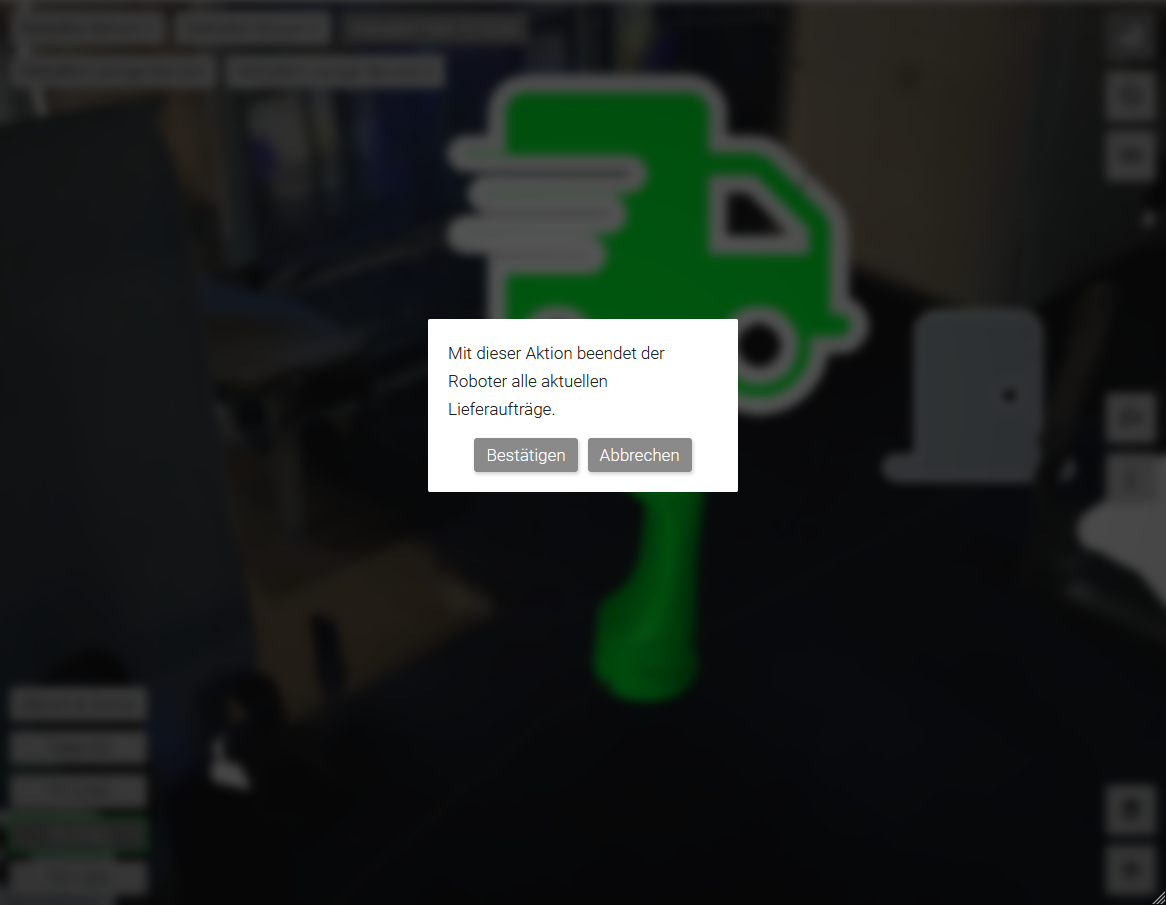
\includegraphics[width=0.9\textwidth]{Screenshot Dialog.png}
    \\
    Quelle: Eigene Darstellung
\end{figure}

In der fünften Regel geht es darum, dass Aktionen, die Fehler auslösen, verhindert werden sollten \cite[Regel 5]{Nielsen.1994}. In der Steuerung ist es zum Beispiel nicht möglich, ungültige Standorte in der Routenplanung einzugeben. Währenddessen wird diese Regel in der Verwaltung durch die bereits erwähnten Bestätigungsdialoge erfüllt. Im Editiermodus gibt es die bereits erwähnte Rückgängigmachen- und Wiederholen-Funktion.

In der siebten Regel geht darum, dass bestimmte, häufig genutzte Aktionen durch Shortcuts schneller ausführbar sein sollten \cite[Regel 7]{Nielsen.1994}. So können Zielstandort und Roboter für einen Lieferauftrag in der Steuerung sowohl über die Inputs als auch über die Karte ausgewählt werden. Im Editiermodus gibt es außerdem Tastenkombinationen für das Rückgängigmachen und Wiederholen.

Auch die anderen Usability Entscheidungsregeln wurden während der Entwicklung beachtet und weitestgehend erfüllt, was aber nicht automatisch bedeutet, dass der Prototyp auch wirklich benutzerfreundlich ist. Um das zu bewerten, folgen die Usability Tests.

\subsubsection{Usability Tests}\label{sec:UsabilityTests}
Während eines Großteils der Implementierung wurde die Benutzerfreundlichkeit nur oberflächlich durch den Entwickler bewertet, wodurch viel Zeit gespart wurde. Da sich die Entwickler von Systemen nicht zum Testen ebendieser eignen, konnten viele Probleme allerdings nicht identifiziert werden. Aus diesem Grund wurden Usability Tests mit ausgewählten Testpersonen durchgeführt, nachdem alle Funktionen des Prototyps erfolgreich implementiert wurden. Da die Benutzerfreundlichkeit des fertigen Prototyps bewertet werden soll und ein Vergleich zu vorherigen Versionen unwichtig ist, wurden qualitative statt quantitative Usability Tests durchgeführt.

Der Aufbau der Usability Tests basiert maßgeblich auf verschiedenen Artikeln der Nielsen Norman Group. So wurden die Aufgaben nach dem Stepped-User-Tasks-System \cite{Pernice.2020} formuliert und während der Durchführung der Tests wurde darauf geachtet, dass die Testpersonen die Thinking-Aloud-Methode \cite{Nielsen.2012b} einsetzen. Die Usability Tests wurden in zwei Runden mit jeweils fünf Personen durchgeführt. So konnten die gefundenen Probleme nach der ersten Runde behoben werden, bevor die zweite Runde durchgeführt wurde. Für die Usability Tests wurden drei Aktivitäten vorbereitet, die die Testpersonen nacheinander durchführen sollten. Die Aktivitäten decken direkt oder indirekt einen großen Teil der Funktionen des Prototyps ab. Konkret beschäftigen sich die Aktivitäten mit der Übersicht, der Steuerung und dem Editiermodus, aber nicht mit der Verwaltung. In der ersten Aktivität müssen Position und Akkustand eines bestimmten Roboters gefunden werden. Daraufhin muss der Roboter in der zweiten Aktivität zu einem oder mehreren Standorten und dann zurück zur Ladestation geschickt werden. In der dritten Aktivität muss ein 3D-Modell mithilfe des Editiermodus richtig positioniert werden. In der dritten Aktivität wird beispielsweise nicht nur geprüft wie Benutzerfreundlich das Editieren ist, sondern auch wie leicht der Editiermodus überhaupt gefunden werden kann.

Um die geplanten Aktivitäten zu prüfen, wurde zunächst ein Pilottest durchgeführt. Mithilfe von Pilottests können Probleme im Design von Tests gefunden werden, sodass diese vor der Durchführung der richtigen Tests aus dem Weg geschafft werden können \cite{Schade.2015}. Mithilfe des Pilottests konnten die Aktivitäten optimiert werden. Außerdem konnten die Ergebnisse des Pilottests bezüglich der Benutzerfreundlichkeit des Prototyps ausgewertet werden, sodass viele Probleme behoben werden konnten, bevor die anderen Tests durchgeführt wurden.

\paragraph{Erster Testdurchlauf}

In den beiden folgenden Tabellen werden die Ergebnisse des ersten Usability Testdurchlaufs zusammengefasst. Der Pilottest wird zu dieser Runde dazugezählt und ist in den Tabellen als T0 gekennzeichnet. In Tabelle \ref{tbl:1stUsabilityTestsProblems} wird dargestellt, welche Probleme bei welcher Testperson aufgefallen sind. So sieht man, dass die meisten Probleme die im Pilottest aufgefallen sind, danach nicht mehr aufgetreten sind, was darauf zurückzuführen ist, dass diese vor der Durchführung der restlichen Tests behoben wurden. Man kann zudem sehen, dass den meisten Testpersonen mindestens ein Problem aufgefallen ist, das keiner anderen Testperson aufgefallen ist. Hierdurch zeigt sich, dass durch weniger Testpersonen weniger Probleme gefunden worden wären. In Tabelle \ref{tbl:1stUsabilityTestsProblemsDesc} im Anhang werden die gefundenen Probleme genauer beschrieben. Bei der Korrektur der Probleme wurden die Probleme priorisiert, die besonders vielen Testpersonen aufgefallen sind. Im Rahmen der Usability Tests gab es außerdem zusätzlich Feedback der Testpersonen, das in der folgenden Implementierungsphase berücksichtigt wurde.

\begin{table}[H]
    \caption{Gefundene Probleme in erster Usability Testrunde}\label{tbl:1stUsabilityTestsProblems}
    \begin{tabular}{l|l|l|l|l|l|l}
                & T0    & T1    & T2    & T3    & T4    & T5    \\ \hline
    Problem 1   & X     &       &       & X     &       &       \\
    Problem 2   & X     &       &       &       &       &       \\
    Problem 3   & X     &       &       &       &       &       \\
    Problem 4   & X     &       &       &       &       &       \\
    Problem 5   & X     &       &       &       &       &       \\
    Problem 6   & X     &       & X     &       &       &       \\
    Problem 7   & X     &       &       &       &       &       \\
    Problem 8   & X     &       &       &       & X     &       \\
    Problem 9   &       & X     &       &       &       &       \\
    Problem 10  &       & X     &       &       &       &       \\
    Problem 11  &       & X     & X     & X     & X     &       \\
    Problem 12  & X     & X     & X     &       &       &       \\
    Problem 13  &       &       & X     &       &       &       \\
    Problem 14  &       &       & X     & X     &       &       \\
    Problem 15  & X     &       & X     &       &       &       \\
    Problem 16  &       &       &       & X     &       &       \\
    Problem 17  &       &       &       & X     &       &       \\
    Problem 18  &       &       &       &       &       & X     \\
    Problem 19  &       &       &       &       &       & X     \\
    Problem 20  &       &       &       &       &       & X     \\
    \end{tabular}    
\end{table}

In Tabelle \ref{tbl:1stUsabilityTestsActions} sind die Aktivitäten in verschiedene Aktionen aufgeteilt, die bei der Ausführung der Aktivität durchgeführt werden können, aber nicht unbedingt durchgeführt werden müssen. Die Werte zeigen, wie gut eine Aktion von einer Testperson durchgeführt werden konnte. Je niedriger der Wert, desto besser konnten die Aktionen durchgeführt werden. Kein Wert bedeutet, dass die Testperson die Aktion nicht durchgeführt hat, da sie für den Erfolg der Aktivität nicht benötigt wurde. Aus der Tabelle wird somit die Benutzerfreundlichkeit in den entsprechenden Teilen der Anwendung ersichtlich. Man sieht, dass die meisten Aktionen nach dem Pilottest deutlich besser durchgeführt werden konnten, was auf die erwähnten Anpassungen am Prototyp zurückzuführen ist. Die Tabelle zeigt, dass die meisten Aktionen zuverlässig durchgeführt werden können, sie zeigt aber auch, dass die Benutzerfreundlichkeit an einigen Stellen noch ausbaufähig ist. Insbesondere der Editiermodus hat Mängel, aber auch in der Übersicht und Steuerung gibt es kleinere Probleme.


\begin{table}[H]
    \caption{Bewertung der durchgeführten Aktionen in erster Usability Testrunde}\label{tbl:1stUsabilityTestsActions}
    \begin{tabular}{l|llllll}
        Aktion                              & T0        & T1        & T2        & T3        & T4        & T5        \\ \hline
        \textbf{Aktivität 1 (Übersicht)}    &           &           &           &           &           &           \\
        Roboter mit Button ausgewählt       &         1 &         1 &         1 &         1 &         1 &         1 \\
        Akkustand gefunden                  &         2 &         1 &         1 &         2 &         2 &         1 \\
        Roboter mit Folgen-Button gefunden  &         2 &         1 &         1 &         - &         - &         - \\
        Roboter mit Karte gefunden          &         - &         - &         - &         2 &         1 &         1 \\ \hline

        \textbf{Aktivität 2 (Steuerung)}    &           &           &           &           &           &           \\
        Lieferauftrag-Button gefunden       &         1 &         1 &         1 &         1 &         1 &         1 \\
%       Roboter mit Karte ausgewäht         &         - &         - &         - &         - &         - &         1 \\
        Standort mit Personfinder ausgewählt&         2 &         - &         1 &         1 &         1 &         1 \\
        Standort mit Karte ausgewählt       &         - &         1 &         - &         - &         1 &         1 \\
        Lieferauftrag gestartet             &         3 &         2 &         1 &         1 &         1 &         1 \\
        Roboter zur Ladestation geschickt   &         - &         1 &         1 &         1 &         1 &         1 \\ \hline

        \textbf{Aktivität 3 (Editiermodus)} &           &           &           &           &           &           \\
        Editormodus über Adminansicht       &         3 &         - &         - &         - &         - &         - \\
        Editormodus über Nutzeransicht      &         - &         1 &         1 &         1 &         1 &         1 \\
        Steuerung verstanden                &         - &         1 &         3 &         1 &         2 &         1 \\
        Undo/Redo genutzt                   &         - &         - &         - &         - &         - &         - \\
        Modell positioniert                 &         2 &         1 &         2 &         1 &         1 &         1 \\
    \end{tabular}
\end{table}


\paragraph{Zweiter Testdurchlauf}

Die Ergebnisse der ersten Usability Tests Runde wurden in der darauffolgenden Implementierungsphase einbezogen. Verschiedene Probleme wurden behoben und das Feedback wurde umgesetzt. Daraufhin wurde eine neue Runde an Usability Tests mit fünf neuen Testpersonen durchgeführt. Die Ergebnisse sind in den folgenden zwei Tabellen abgebildet. Die Tabellen folgen der Struktur der vorherigen Tabellen. So zeigt Tabelle \ref{tbl:2ndUsabilityTestsProblems}, welche Testperson welche Probleme hatte und Tabelle \ref{tbl:2ndUsabilityTestsActions} wie gut Aktionen durchgeführt werden konnten. In Tabelle \ref{tbl:2ndUsabilityTestsProblemsDesc} im Anhang werden die gefundenen Probleme beschrieben. 

Man sieht in Tabelle \ref{tbl:2ndUsabilityTestsProblems}, dass deutlich weniger Probleme aufgefallen sind. Neben den Problemen gab es auch noch weiteres Feedback, dass sich aber vor allem auf Rechtschreibung, Zeichensetzung und Benennung beschränkt. Außerdem ist aus dem Feedback erkenntlich, dass das erste Auffinden von bestimmten Funktion etwas dauern kann, die Bedienung dieser Funktionen dann aber einwandfrei funktioniert. Es ist zu erwarten, dass die Bedienung des Prototyps bei einer erneuten Nutzung deutlich leichter ist, da die Funktionen dann nicht mehr lange gesucht werden müssen.

\begin{table}[H]
    \caption{Gefundene Probleme in zweiter Usability Testrunde}\label{tbl:2ndUsabilityTestsProblems}
    \begin{tabular}{l|l|l|l|l|l}
                    & T1    & T2    & T3    & T4    & T5    \\ \hline
        % Beim entfernen der Roboter Auswahl wird fälschlicherweise in das Stockwerk des Roboters gewechselt bei dem die Auswahl entfernt wurde
        Problem 1   & X     &       &       &       &       \\
        % Steuerungsbuttons müssen nicht immer aktiv sein (Abbrechen, wenn kein Lieferauftrag existiert; Laden, wenn bereits geladen wird)
        Problem 2   & X     &       &       &       &       \\
        % Roboter kann nicht über die Karte (ohne den "zur Ladestation" Button) zur Ladestation geschickt werden
        Problem 3   &       & X     &       &       &       \\
        % Suchfunktion von Standorten wurde nicht gefunden, weil diese im Lieferauftrag versteckt ist
        Problem 4   &       &       & X     &       &       \\
        % Irritation, dass Erklärung der Steuerung im Tooltip steht und nicht einfach permanent angezeigt an einer anderen Position angezeigt wird
        Problem 5   &       &       &       & X     &       \\
        % Editiermodus im Admin-Modus nicht gefunden
        Problem 6   &       &       &       &       & X     \\
        % Editiermodus im Nutzermodus nicht gefunden
        Problem 7   &       &       &       &       & X     \\
    \end{tabular}    
\end{table}

Auch in Tabelle \ref{tbl:2ndUsabilityTestsActions} fällt auf, dass deutlich weniger Probleme aufgetreten sind. So gab es nur bei der zweiten und fünften Testperson geringfügige bis erhebliche Probleme. Die zweite Testperson hatte erst versucht den Roboter direkt über eine Auswahl auf der Karte zur Ladestation zu schicken, während die fünfte Testperson Probleme damit hatte, den Editiermodus zu finden, wobei hierfür ohne Erfolg in der Verwaltung gesucht wurde, bevor der Editiermodus in der Nutzeransicht gefunden wurde. So handelt es sich um Probleme, die bei einer erneuten Nutzung der Anwendung nicht mehr auftreten würden. Nachdem die Tests ausgewertet wurden, wurde der Prototyp erneut angepasst, wodurch die beiden genannten Probleme nicht mehr auftreten sollten. Auch die in Tabelle \ref{tbl:2ndUsabilityTestsProblems} aufgelisteten Probleme wurden behoben.

\begin{table}[H]
    \caption{Bewertung der durchgeführten Aktionen in zweiter Usability Testrunde}\label{tbl:2ndUsabilityTestsActions}
    \begin{tabular}{l|lllll}
        Aktion                              & T1    & T2    & T3    & T4    & T5    \\ \hline
        \textbf{Aktivität 1 (Übersicht)}    &       &       &       &       &       \\
        Roboter mit Button ausgewählt       & 1     & 1     & 1     & 1     & 1     \\
        Akkustand gefunden                  & 1     & 1     & 1     & 1     & 1     \\
        Roboter mit Folgen-Button gefunden  & -     & -     & -     & -     & -     \\
        Roboter mit Karte gefunden          & 1     & 1     & 1     & 1     & 1     \\ \hline
        \textbf{Aktivtiät 2 (Steuerung)}    &       &       &       &       &       \\
        Lieferauftrag-Button gefunden       & 1     & -     & -     & -     & 1     \\
%       Roboter mit Karte ausgewäht         & -     & -     & -     & -     & -     \\
        Standort mit Personfinder ausgewählt& 1     & -     & -     & -     & 1     \\
        Standort mit Karte ausgewählt       & -     & 1     & 1     & 1     & -     \\
        Lieferauftrag gestartet             & 1     & 1     & 1     & 1     & 1     \\
        Roboter zur Ladestation geschickt   & 1     & 2     & 1     & 1     & 1     \\ \hline
        \textbf{Aktivität 3 (Editiermodus)} &       &       &       &       &       \\
        Editormodus über Adminansicht       & -     & -     & -     & -     & 3     \\
        Editormodus über Nutzeransicht      & 1     & 1     & 1     & 1     & 2     \\
        Steuerung verstanden                & 1     & 1     & 1     & 1     & 1     \\
        Undo/Redo genutzt                   & -     & -     & 1     & -     & 1     \\
        Modell positioniert                 & 1     & 1     & 1     & 1     & 1     \\
    \end{tabular}
\end{table}

Da die Menge der gefundenen Probleme mit dem zweiten Durchlauf der Tests stark abgenommen hat und da die Aktivitäten fast ohne Probleme durchgeführt wurden, wurde auf einen dritten Durchlauf verzichtet. Es ist nicht zu erwarten, dass ein dritter Durchlauf bedeutende neue Erkentnisse liefern würde, da aufgrund der Ergebnisse der vorherigen Tests angenommen werden kann, dass nur noch wenige Probleme bestehen, die auch mit einem erneuten Durchlauf nicht unbedingt gefunden werden können. Es ist wichtig zu beachten, dass mit den Usability Tests nicht alle Funktionen des Prototyps getestet wurden. Stattdessen wurden nur die wichtigsten Funktionen getestet die mit \deckgl{} in Verbindung stehen und somit für die Forschungsfrage dieser Arbeit größere Relevanz haben. Ob die Liste der Roboter und Stockwerke in der Verwaltung besonders Benutzerfreundlich ist, ist für die Forschungsfrage nicht so relevant, da die Liste sehr simpel ist und keine besonderen Technologien nutzt. In Kombination mit der Einhaltung der Usability Entscheidungsregeln ist davon auszugehen, dass das Ziel der Benutzerfreundlichkeit ausreichend erfüllt wurde.

\subsection{Effizienz}
Wie im Abschnitt \ref{sec:PerformanceBasics} beschrieben werden \ac{PLS}, \ac{LR} und Smoothness bewertet. Für die Bestimmung des \ac{PLS} wird der \ac{FCP} gemessen. Normalerweise wird zur Bestimmung des \ac{PLS} der \ac{LCP} gemessen, was aber nicht möglich ist, da die Ladezeit des wichtigsten Elements – der \deckgl{} Karte – nicht gemessen werden kann. Die \ac{LR} wird über den \ac{FID} und die \ac{TBT} gemessen. Die Smoothness wird auf Basis von Beobachtungen während der Usability Tests bestimmt, da die \ac{INP} durch den Einsatz von \deckgl nicht gemessen werden kann. Die Messwerte wurden über die in Webbrowser integrierte PerformanceObserver-\ac{API} \cite{PerformanceObserver} gemessen. Die gemessenen Werte Stammen von einer Auswahl von Personen die mit dem Prototyp interagieren sollten.

% FCP 24 Werte
% Mittelwert: 760 ms
% Median: 743 ms
% Min: 430 ms
% Max: 1806 ms
% < 1800 gut; > 3000 poor

% FID 13 Werte (weniger weil Wert nicht in allen Browsern gemessen wird)
% Mittelwert: 138 ms
% Median: 3 ms
% Min: 1 ms
% Max: 1751 ms
% < 100 gut; > 300 poor

% TBT 23 Werte
% Mittelwert: 860 ms
% Median: 605 ms
% Min: 25 ms
% Max: 2678 ms
% < 200 gut; > 600 poor

\subsubsection{Effizienzmesswerte}

In Abbildung \ref{fig:EfficiencyBoxplot} werden die Ergebnisse in mehreren Boxplot-Diagrammen dargestellt. Es wurden insgesamt 24 \ac{FCP}-, 13 \ac{FID}- und 23 \ac{TBT}-Werte gemessen. Die Differenz in der Menge ist darauf zurückzuführen, dass der \ac{FID} nicht in allen Webbrowsern gemessen werden kann und dass die Anwendung wieder geschlossen werden kann, nachdem der \ac{FCP} gemessen wurde, aber bevor die \ac{TBT} gemessen wurde. Wie an sieht, liegt der Mittelwert beim \ac{FCP} bei 760 ms und der Median bei 743 ms. Außerdem gibts einen Ausreißer der bei 1806 ms liegt. Beim \ac{FID} liegen alle Werte bis auf einen Ausreißer – der bei 1751 ms liegt – bei unter 10 ms. Durch den Ausreißer gibt es eine große Differenz zwischen Mittelwert und Median. So ist der Mittelwert 138 ms während der Median 3 ms ist. Die \ac{TBT} Werte liegen breit verteilt zwischen 25 ms und 2678 ms. Der Mittelwert ist 860 ms und der Median ist 605 ms.

\begin{figure}[H]
    \caption{Effizienzmesswerte}\label{fig:EfficiencyBoxplot}
    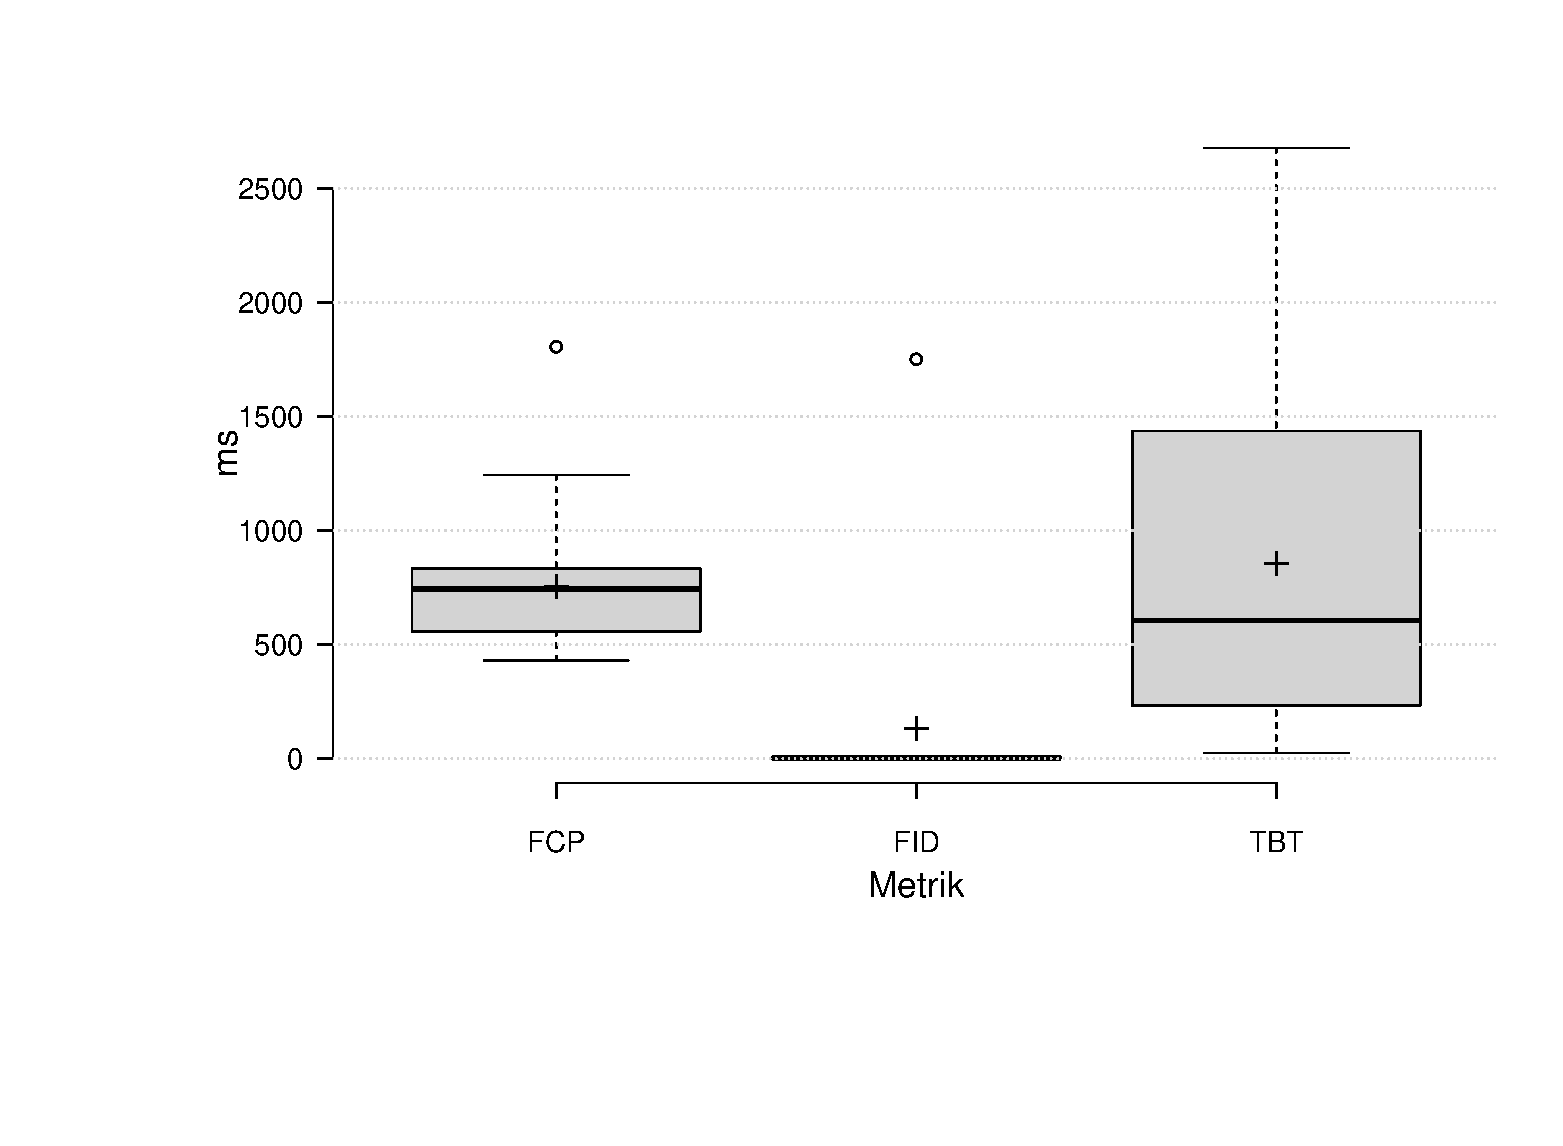
\includegraphics[width=0.9\textwidth]{Boxplot.pdf}
    \\
    Quelle: Eigene Darstellung
\end{figure}


\subsubsection{Bewertung der Effizienz}
Solange der \ac{FCP} unter 1800 ms liegt, kann dieser als gut bewertet werden \cite{FCP}. Die gemessenen \ac{FCP} Werte liegt bis auf den Ausreißer unter diesem Richtwert. Für eine gründliche Bewertung des \ac{PLS} reicht dieser Messwert nicht aus, da die Ladezeit der Kartenansicht nicht gemessen wird. Trotzdem kann zumindest der \ac{PLS} der \ac{GUI}-Elemente als gut bewertet werden.

Bis auf einen Ausreißer liegen alle gemessenen \ac{FID}-Werte unter dem Richtwert von 100 ms \cite{FID}, was bedeutet, dass die erste Interaktion in der Regel eine geringe Latenz hat. Gleichzeitig liegt die \ac{TBT} über dem Mindestwert von 600 ms \cite{TBT}, was bedeutet, dass der Hauptthread lange blockiert wird, sodass Interaktionen während des Ladens der Kartenansicht eine hohe Latenz haben. Diese Messwerte erscheinen auf den ersten Blick widersprüchlich, lassen sich aber dadurch erklären, dass die Karte während des Ladevorgangs keine Daten anzeigt, wodurch es keinen Anreiz gibt mit der Anwendung zu interagieren. Erst wenn die Kartenansicht vollständig geladen wurde und der Hauptthread nicht mehr blockiert wird, wird der Inhalt angezeigt. So interagieren die meisten Nutzer erst mit der Anwendung, wenn der Hauptthread nicht mehr blockiert wird, wodurch die Latenz der Interaktionen gering ist. Die \ac{LR} ist somit schlecht, was sich allerdings nicht negativ für den Nutzer auswirkt, da dieser sowieso erst mit der Anwendung interagiert, nachdem die Kartenansicht vollständig geladen wurde.

Während der Usability Tests konnten keine Ruckler beobachtet werden und auch außerhalb der Usability Tests sind bei der Nutzung des Prototyps keine Ruckler aufgefallen. Insgesamt erscheint die Bedienung der Kartenansicht sowohl am Desktop als auch an Mobilgeräten flüssig. Daher kann die Smoothness als gut bewertet werden. Es gilt natürlich zu beachten, dass diese Bewertung nicht auf objektiven Messwerten, sondern nur auf subjektiven Beobachtungen basiert.

Zusammenfassend lässt sich die Effizenz der Anwendung als ausreichend bewerten.


% => Performance Tests (testen welche Maßnahmen welche Performance Auswirkungen haben)
% Maßnahmen
% Nutzung des .glb Formats statt .obj (beides mit und ohne Kompression)
    % Einfluss auf Ladezeiten (Netzwerk und Rendering)
    % Einfluss auf GPU und CPU Auslastung
% Caching der Robotermodelle
% Caching aller anderen Anfragen (Bis auf Roboter)
% Sehr Kurzzeitiges Caching der Roboter
% Initialisierung der Karten Vorschau über Button statt beim Öffnen des Aufklappers (vielleicht nicht ganz passend?)
